\documentclass[landscape]{sciposter}

%\documentclass[a0, plainboxedsection, landscape]{sciposter}

\usepackage{multicol}
\usepackage{sectionbox}
\usepackage{graphicx}
\usepackage{subfig}
\usepackage{amsmath}
\usepackage{siunitx}
\usepackage{caption}
\usepackage[euler]{textgreek}

\renewcommand{\papertype}{custom}
%\renewcommand{\fontpointsize}{32 pt}
\setlength{\paperwidth}{48 in}
\setlength{\paperheight}{36 in}
\renewcommand{\setpspagesize}{
	\ifthenelse{\equal{\orientation}{landscape}}{
		\special{papersize=36 in, 48 in}
	}{\special{papersize=48 in, 36 in}
	}
}

\setmargins[5.5cm]
\leftlogo[0.75]{colby.jpg}
\norightlogo

\title{Millimeter-wave precision spectroscopy of potassium in Rydberg states}
\author{Charles Conover, Huan Bui '21}
\institute{Department of Physics and Astronomy, Colby College, Waterville, Maine}
\conference{DAMOP - Milwaukee, Wisconsin - May 27 - 31, 2019}
%\sectionfont{\fontsize{32 pt}{40 pt}\selectfont}

\begin{document}
%\renewcommand{\titlesize}{\Huge}
\renewcommand{\titlesize}{\fontsize{64 pt}{80 pt}\selectfont}
\renewcommand{\authorsize}{\fontsize{40 pt}{50 pt}\selectfont}
\renewcommand{\instsize}{\fontsize{40 pt}{50 pt}\selectfont}
\maketitle

\fontsize{32 pt}{40 pt}\selectfont

\begin{multicols}{4}
\setlength{\columnseprule}{0pt}

\section*{\large Abstract}
{\normalfont We measure mm-wave transitions between Rydberg states in $^{\text{39}}$K to a part in 10\textsuperscript{7} to determine d-state quantum defects and absolute energy levels of potassium. $^{\text{39}}$K atoms are magneto-optically trapped and cooled to 1 mK, and excited from ground state 4s\textsubscript{1/2} to nd\textsubscript{3/2} or nd\textsubscript{5/2} by frequency-stabilized 405 nm and 980 nm ECDL's in succession. The nd $\rightarrow$ (n+1)d transitions are driven by a \textmu s-long pulse of mm-wave before the atoms are selectively ionized for detection. The (n+1)d population is measured as a function of mm-wave frequency. Static electric fields in the MOT are nulled in three dimensions to eliminate DC Stark shifts. Zero AC Stark shift resonance frequencies are extrapolated from non-zero AC Stark shift measurements, or measured directly without extrapolation with a double mm-wave pulse of width $\tau$ and scanning delay $T$ (Ramsey SOF technique).}

\begin{figure}
\begin{center}
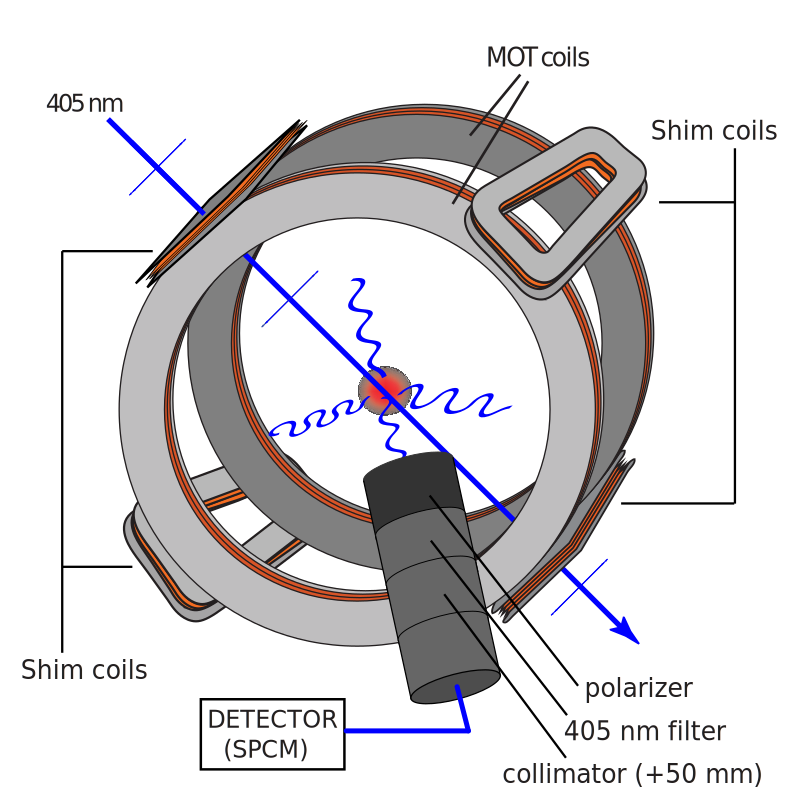
\includegraphics[scale = 0.90]{MOT.png}
%\normalfont{\caption{}}
%\label{Figure 1}
\end{center}
\end{figure}

\normalfont{The MOT cloud is trapped in a magnetic field and cooled by a 770 nm laser (not shown). The rods provide a static field and an ionization field. A mm-wave drives nd $\rightarrow$ (n+1)d transitions.}

\begin{figure}
\begin{center}
\includegraphics[scale = 0.95]{excitation.png}
%\normalfont{\caption{}}
%\label{Figure 2}
\end{center}
\end{figure}

\normalfont{(a) Trapping and excitations from 4s\textsubscript{1/2} to nd states in 2 steps. (b) Two-photon mm-wave transitions and their approximate frequencies.}

\section*{\large Static field elimination}
Energy levels at highly excited states are sensitive to external static electric fields. Measured nd $\rightarrow$ (n+1)d transition frequencies vary quadratically with the static field amplitude:
\begin{equation*}
\resizebox{0.65\hsize}{!}{$\Delta \nu_{nd \rightarrow (n+1)d} = \nu_{0} - \frac{1}{2} \Delta \alpha E^2$},
\end{equation*}
where $\Delta \alpha$ is the difference between the (n+1)d and nd polarizabilities. In general, $\alpha$ represents how strongly energy levels shift in response to an external static electric field. 

\begin{figure}
\begin{center}
\includegraphics[scale = 0.8]{33d52_deltaV_population.eps}
\includegraphics[scale = 0.8]{33d52_DeltaV.eps}
\includegraphics[scale = 0.8]{33d52_Vy.eps}
\includegraphics[scale = 0.8]{33d52_VSum.eps}
%\caption{\normalfont{}}
%label{Figure 3}
\end{center}
\end{figure}

Static field elimination for 33d\textsubscript{5/2} $\rightarrow$ 34d\textsubscript{5/2} transition. Shown are 34d\textsubscript{5/2} population distributions and transition frequencies at different static field values in orthogonal directions. Projected maximum frequency in one direction corresponds to a DC bias that nullifies the field in that direction.

\section*{\large Zero mm-wave power extrapolation}
While not a large effect, the energy shift caused by the mm-wave source is significant at our level of precision. This shift is directly proportional to the intensity of the interacting mm-wave. 

\begin{figure}
\begin{center}
\includegraphics[scale = 1.25]{33d52_PScans.eps}
%\caption{\normalfont{}}
%\label{Figure 4}
\end{center}
\end{figure}

Zero-power extrapolation for 33d\textsubscript{5/2} $\rightarrow$ 34d\textsubscript{5/2} transition after static field elimination. The y-intercept of the linear fit of the measured transition frequencies is the mm-wave-free transition frequency. The energy shifts from 0.35 to 0 relative intensity are on the order of a few kHz.\\

The 33d\textsubscript{5/2} $\rightarrow$ 34d\textsubscript{5/2} spacing can then be calculated:
\begin{align*}
\Delta \nu_0 = \textrm{2f\textsubscript{mm}} &= \textrm{179,496 MHz - 12.540 MHz} \\ &= \textrm{179,483.46 MHz}
\end{align*}

\section*{\large Determination of d-state quantum defects}
The absolute energies are given by:
\begin{equation*}
\resizebox{0.45\hsize}{!}{$E_n = -\frac{hcR_K}{(n - \delta(n))^2},$}
\end{equation*}
where $n$ is the principal quantum number, and $\delta(n)$ is parameterized by two coefficients, $\delta_0$ and $\delta_2$, as:
\begin{equation*}
\resizebox{0.5\hsize}{!}{$\delta(n) = \delta_0 + \frac{\delta_2}{(n-\delta_0)^2}.$}
\end{equation*}

\begin{figure}
\begin{center}
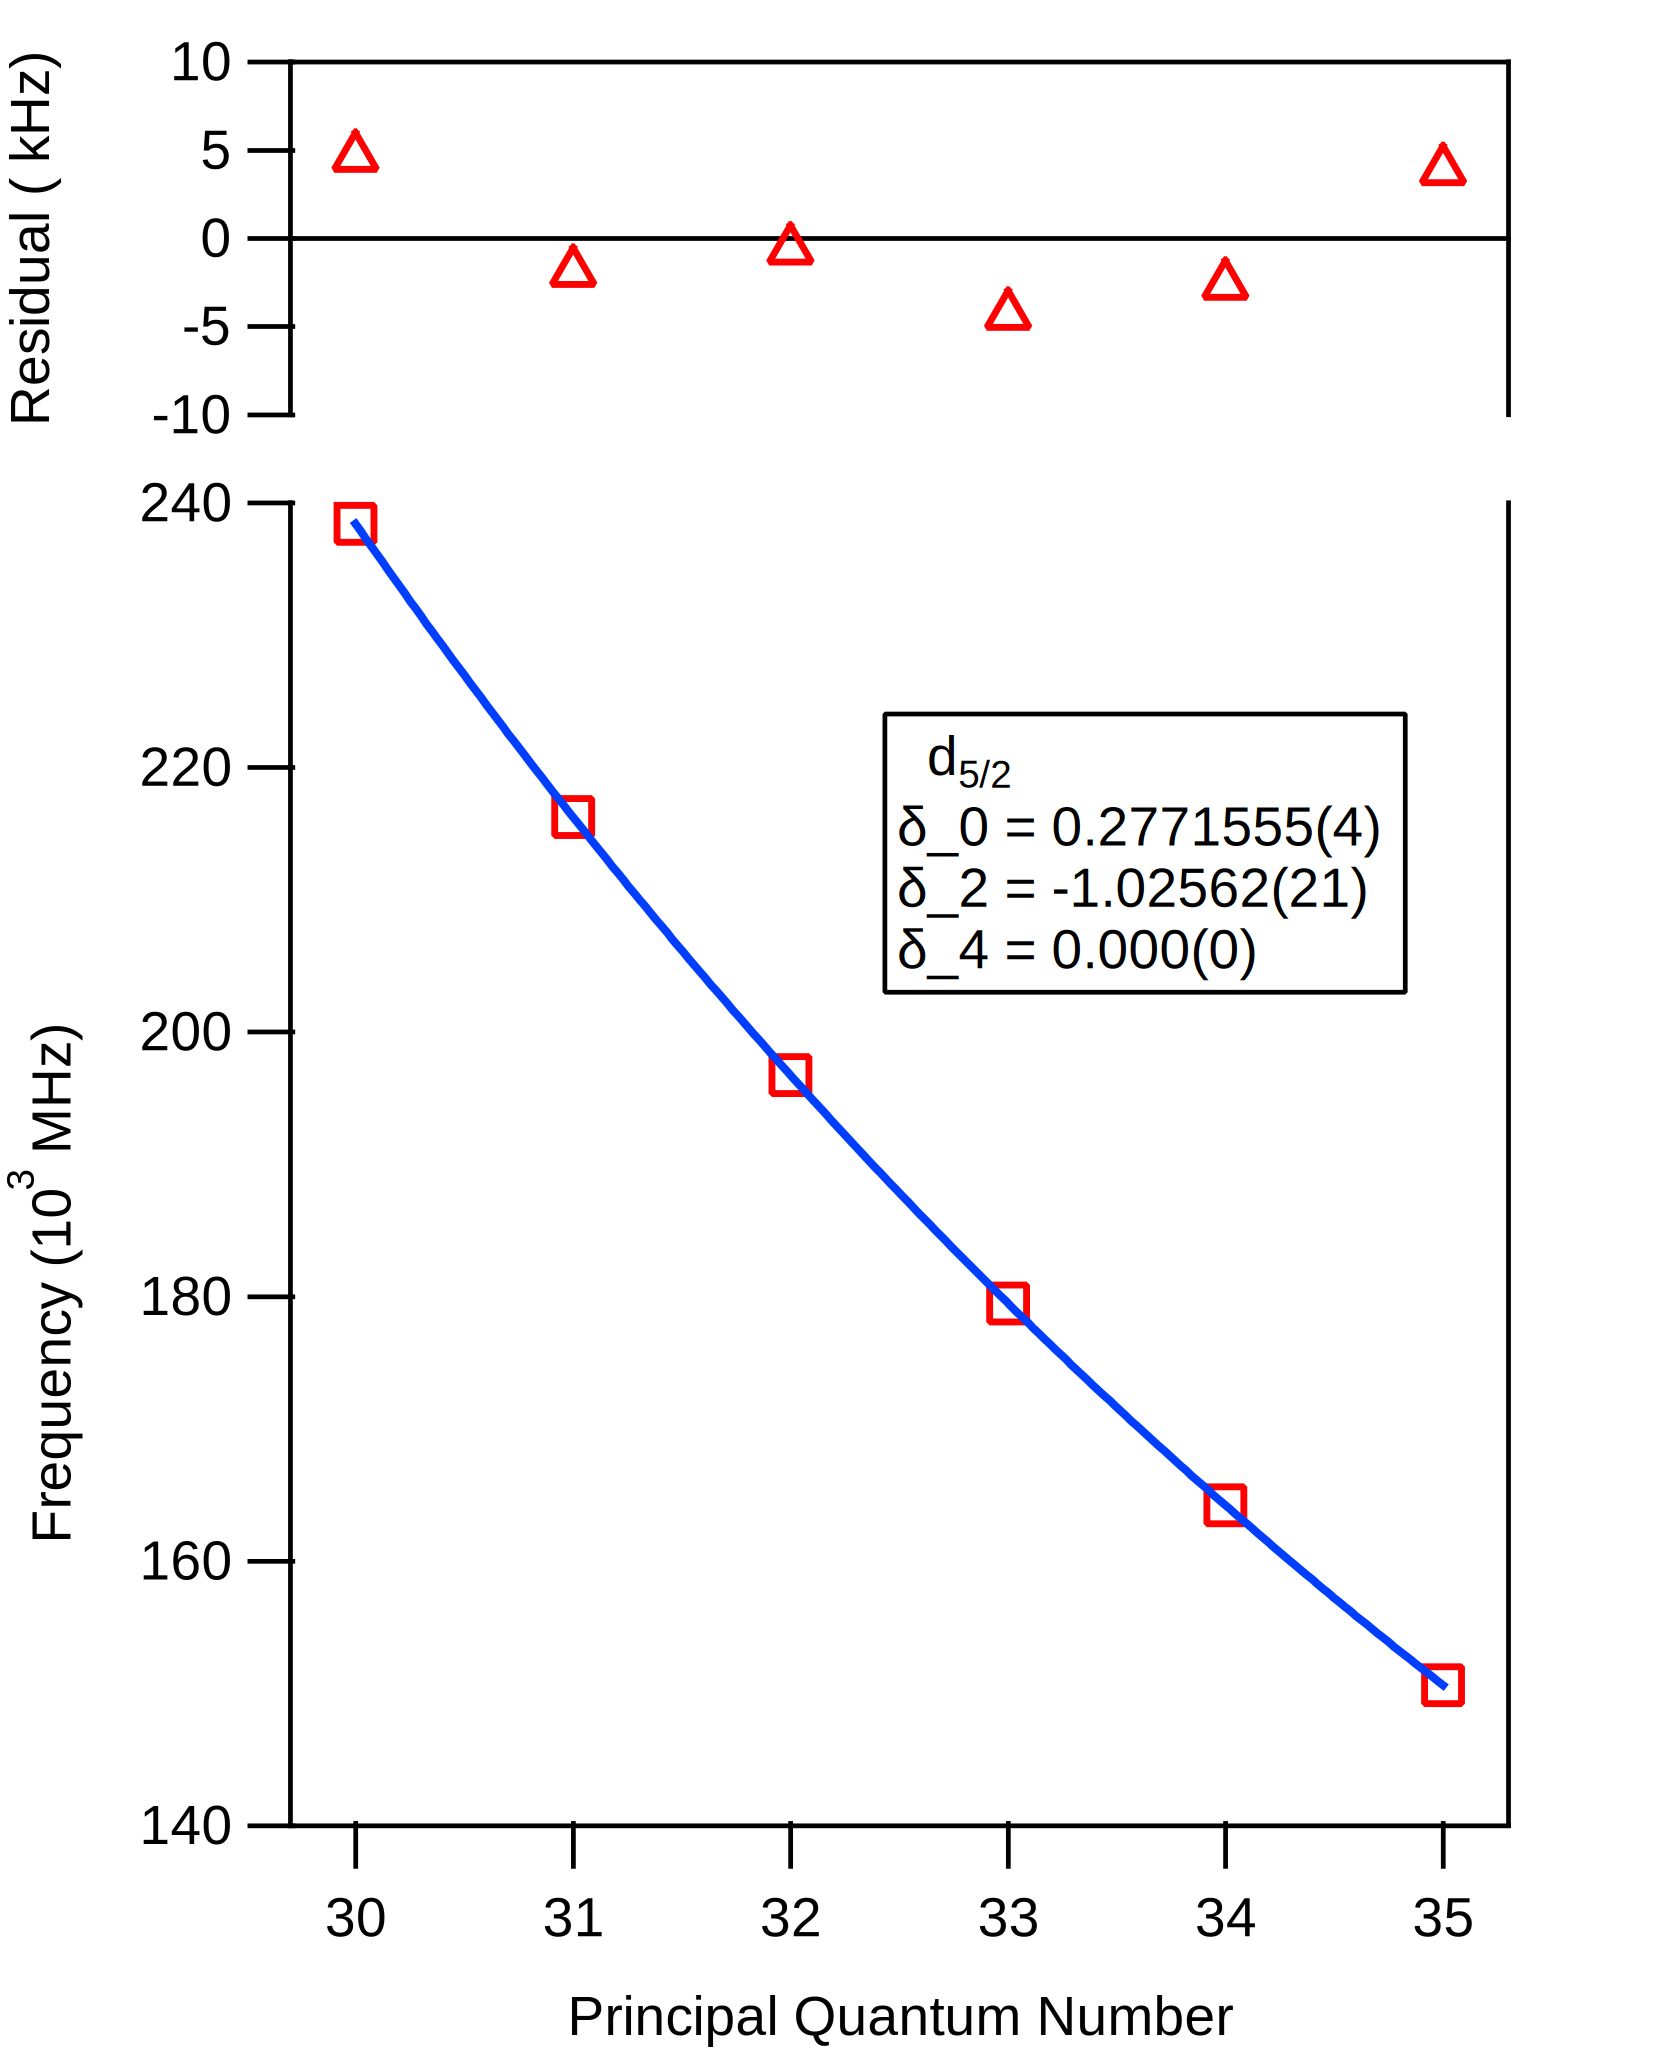
\includegraphics[scale = 0.97]{d32_qd.eps}
\includegraphics[scale = 0.97]{d52_qd.eps}
%\caption{\normalfont{}}
%\label{Figure 5}
\end{center}
\end{figure}

nd $\rightarrow$ (n+1)d transition frequencies versus principal quantum number. A fit of the measured resonance frequencies are used to determine $\delta_0$ and $\delta_2$ for the d\textsubscript{3/2} and d\textsubscript{5/2} states. Residuals of the fit are less than a part in 10\textsuperscript{7} of the transition frequencies.

\section*{\large Ramsey's SOF, an alternative technique}
Ramsey's separated oscillatory field method removes the need for zero-power extrapolation. K atoms in the nd state are exposed to a double pulse of width $\tau$ and delay $T$ instead of a long, single pulse. 

\begin{figure}
\begin{center}
\includegraphics[scale=1]{Ramsey_excitation.png}
%\caption{\normalfont{}}
%\label{Figure 6}
\end{center}
\end{figure}

The final (n+1)d state population oscillates as a function of $T$: 
\begin{equation*}
\resizebox{0.45\hsize}{!}{$P_{(n+1)d} \propto {\cos}^{2}\left(\frac{\Delta_{0} T}{2}\right),$}
\end{equation*}
where $\Delta_0=\omega_0-[E_{(n+1)d}-E_{nd}]/\hbar$ is the beat frequency between the mm-wave frequency and the atomic transition frequency in zero oscillatory field.
 
\begin{figure}
\begin{center}
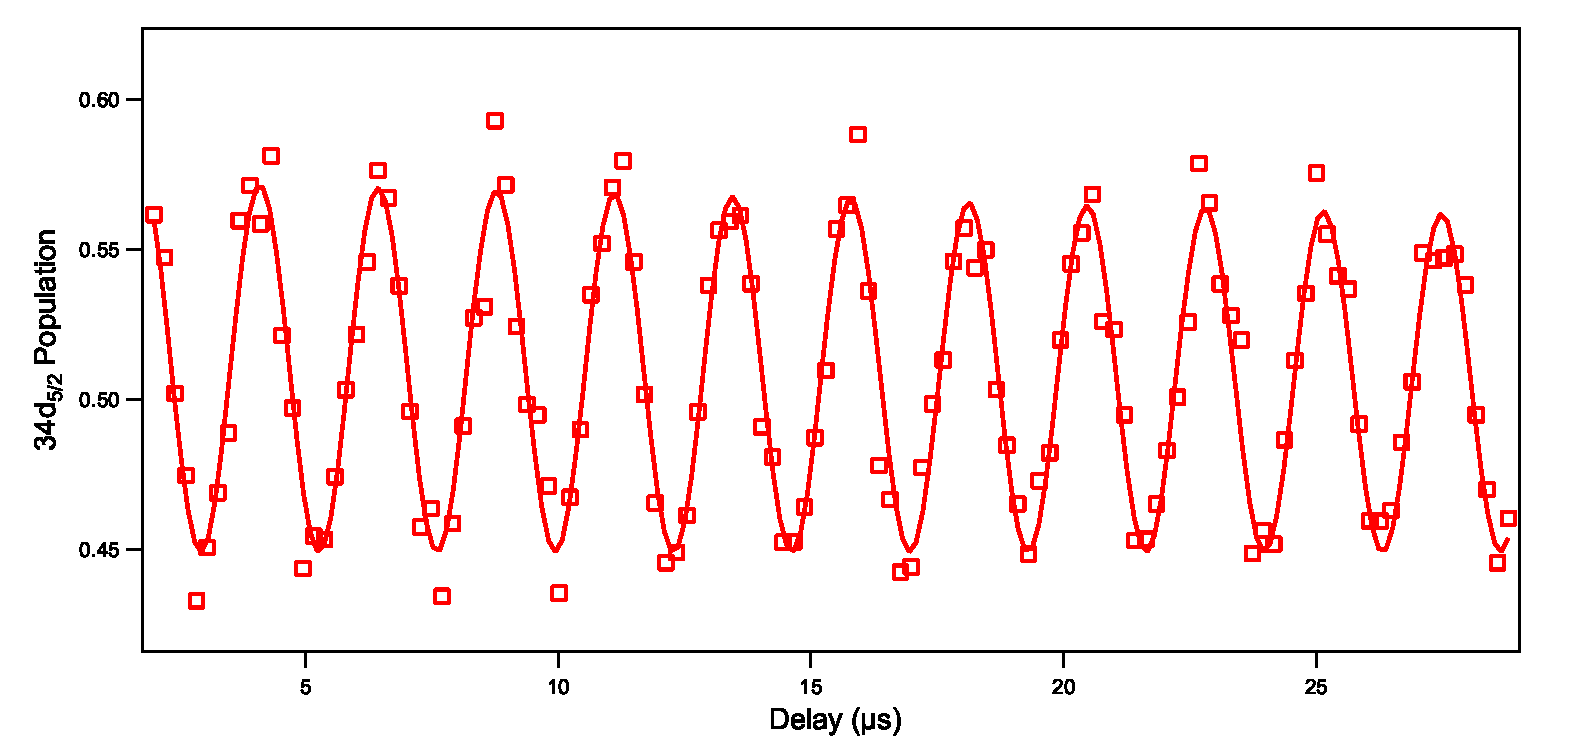
\includegraphics[scale = 1]{33d52_delay_scans.eps}
%\caption{\normalfont{}}
%\label{Figure 7}
\end{center}
\end{figure}

With known mm-wave frequency offset, fitting a cosine squared to a delay scan signal allows for determining the zero-power frequency for the 33d\textsubscript{5/2} $\rightarrow$ 34d\textsubscript{5/2} transition.\\

The fit gives $\Delta_0/2\pi = \textrm{-0.4277 MHz}$. With an initial mm-wave frequency offset of $\textrm{-12.96 MHz}$, the field-free 33d\textsubscript{5/2} $\rightarrow$ 34d\textsubscript{5/2} spacing is:
\begin{align*}
\Delta \nu_0 &= \nu_{\textrm{offset}} - \Delta_0/2\pi + \textrm{179,496 MHz}\\
&= \textrm{-12.96 MHz + 0.4277 MHz + 179,496 MHz} \\ 
&= \textrm{179,483.47 MHz},
\end{align*}
consistent with the zero-power-extrapolated value to within a part in 10\textsuperscript{7}.

\section*{\large Acknowledgments}
This research is supported by Colby College.

\end{multicols}

\end{document}
